
\documentclass[10pt]{beamer}
\usetheme{CambridgeUS}
\usecolortheme{beaver}
\usepackage[utf8]{inputenc}
\usepackage[english]{babel}
\usepackage{amsmath}
\usepackage{amsfonts}
\usepackage{amssymb}
\usepackage{amsthm}		% spezielle theorem Stile
\usepackage{aliascnt} 
\usepackage{tikz}
\usepackage{bm}


\newaliascnt{proposition}{theorem}  
\newtheorem{proposition}[proposition]{Proposition} 
\aliascntresetthe{proposition}

\AtBeginSection[]{
  \begin{frame}
  \vfill
  \centering
  \begin{beamercolorbox}[sep=8pt,center,shadow=true,rounded=true]{title}
    \usebeamerfont{title}\insertsectionhead\par%
  \end{beamercolorbox}
  \vfill
  \end{frame}
}

\author{Mikhail Savelov}
\title{Achieving Equillibria in Vickrey's model}
\subtitle{}
%\setbeamercovered{transparent} 
%\setbeamertemplate{navigation symbols}{} 
%\logo{} 
\institute{University of Passau} 
\date{07.02.2024} 
%\subject{} 


\begin{document}

\begin{frame}

\titlepage

\end{frame}

\begin{frame}
\tableofcontents
\end{frame}

\section{Problem Setting}

\begin{frame}

\begin{itemize}

\item Directed graph $G = (V,E)$, source $s \in V$, destination $t \in V$

\item Planning horizon $[0, \infty)$, time $\theta \geq 0$

\item Strategy space $ \Lambda^{\theta}(r) = \{ h(\theta) \in \mathbb{R}^{\mathcal{P}} |~ \sum_{p' \in \mathcal{P}} h_{p'}(\theta) = r \} $

\item Path-delay operator according to Vickrey's model:
\begin{align*}
\Psi: ( L^2_{+}[0, \theta] )^{\mathcal{P}} &\to ( L^2_{+}[0, \theta] )^{\mathcal{P}} \\
 h &\mapsto \Psi(\cdot, h)
\end{align*}

\item Dynamic equilibrium $h^*(\theta) \in \Lambda^{\theta}(r) $:
  $$ \langle \Psi(\theta, h^*), h^* \rangle \leq \langle \Psi(\theta,  h^*), h \rangle ~\forall h \in  \Lambda^{\theta}(r)  $$

\item Goal: construct a dynamic for $h(\cdot)$, s.t. $$ \lVert \Psi(\theta, h) - \Psi(\theta, h^*) \rVert_2   \stackrel{\theta \to \infty}{\to} 0 $$

\end{itemize}


\end{frame}

\begin{frame}

\begin{figure}
	\begin{center}
		\begin{tikzpicture}[scale=0.2]
			\tikzstyle{every node}+=[inner sep=0pt]
			\draw [black] (7.2,-8.7) circle (3);
			\draw (7.2,-8.7) node {$s$};
			\draw [black] (27.1,-8.7) circle (3);
			\draw (27.1,-8.7) node {$t$};
			\draw [black] (9.808,-7.224) arc (114.62656:65.37344:17.62);
			\fill [black] (24.49,-7.22) -- (23.97,-6.44) -- (23.56,-7.35);
			\draw (17.15,-5.12) node [above] {$\tau_0=1, \nu_0=2$};
			\draw [black] (24.706,-10.5) arc (-58.92949:-121.07051:14.642);
			\fill [black] (24.71,-10.5) -- (23.76,-10.48) -- (24.28,-11.34);
			\draw (17.15,-13.1) node [below] {$\tau_1=2, \nu_1=3$};
		\end{tikzpicture}
		$$ \nu_0 < r < \nu_0 + \nu_1$$
	\end{center}
%	\caption{Two-link network}
\end{figure}

 $$ h^*_0(\theta) = \begin{cases} r , & 0 \leq \theta < \theta^{s} \\  \nu_0, & \theta \geq \theta^s \end{cases} \quad h^*_1(\theta) = r - h^*_0(\theta) $$
 $$\Psi_0(\theta, h^*) = \begin{cases} \tau_0 + \frac{r - \nu_0 }{\nu_0} \theta  , & 0 \leq \theta < \theta^{s} \\  \tau_1,  &\theta \geq \theta^s \end{cases} \quad \Psi_1(\theta, h^*) \equiv \tau_1 $$

$$ \theta^s = (\tau_1 - \tau_0) \frac{\nu_0}{r - \nu_0}$$

\end{frame}


\section{Replicator dynamics}

\subsection{Replicator equation}

\begin{frame}

\begin{itemize}

\item Fitness  $( \phi_p(\theta, h) )_{p \in \mathcal{P}}$, s.t. higher fitness corresponds to "better" path

\item Replicator equation for $p \in \mathcal{P}$:
$$ \dot{h}_p = h_p \cdot K( \phi_p - \overline{\phi} ) $$

 $K > 0$ is a scaling constant,
 $ \overline{\phi}(\theta, h) := \langle \phi(\theta, h), \frac{1}{r} h(\theta) \rangle$ is average fitness  



\item By construction $\sum_{p \in \mathcal{P}} \dot{h_p} = 0 \quad \Rightarrow \quad h(\theta) \in \Lambda^{\theta}(r)$
 
\item We hope to decrease the fitnesses gap by redirecting the inflow to "better" paths

$$ \mathrm{Gap}_\phi (\theta, h) := \max_{h' \in \Lambda^{\theta}(r) } \langle \phi(\theta, h),  h' - h(\theta) \rangle = r ( \phi_{max}(\theta, h) - \overline{\phi}(\theta, h) )$$

\end{itemize}

\end{frame}

\begin{frame}

\begin{itemize}

 \item Integrating the equations allows to write them as Dual Averaging Dynamic:
\begin{align*} 
 y(\theta) &= \log (h(0)) + K \cdot \int_{0}^{\theta} \phi (\theta', h) d\theta'  \\
 h(\theta) &= Q_{\lambda}(y(\theta)) 
\end{align*}


\item $Q_{\lambda}$ is logit choice map on  $\Lambda^{\theta}(r)$:

$$ Q_{\lambda}(v) := \mathrm{arg}\max_{h' \in \Lambda^{\theta}(r)} \left[ \langle v, h' \rangle - \sum_{p \in \mathcal{P}} h'_{p} \log h'_{p} \right] = r \cdot \mathrm{SoftMax}(v)$$

\end{itemize}

\end{frame}


\begin{frame}

\begin{itemize}

\item Condition for correct stabilization: $ \phi(\infty, h^*) = - \Psi(\infty, h^*)  $

%if $h^*$ is the equilibrium, then for $\phi^* = \phi(\infty, h^*)$
%if $x_p > 0, p \in \mathcal{P} \quad \Rightarrow \quad \phi_P = \overline{\phi} $
%$$ \langle \phi^*, h^* \rangle \geq \langle \phi^*, h \rangle \quad \forall h \in \Lambda^{\theta}(r) $$

\item Average delay, true delay, projected delay may be considered as fitnesses

\begin{align*}
	\phi^{\text{avg}}(\theta, h) &:= -\frac{1}{w}\int_{\theta - w}^{\theta} \Psi(\theta', h) d \theta' \\
 	\phi^{\text{true}}(\theta, h) &:= - \Psi(\theta, h) \\
 	\phi^{\text{proj}}(\theta, h) &:= - \left( \Psi(\theta, h) + w  \dot{\Psi}(\theta, h)  \right)
\end{align*}

\item Numerical experiments show that only projected delays lead to convergence
 
\item The Gap function is still not monothone

\end{itemize}

\end{frame}


\subsection{Numerical experiments}

%\begin{frame}
%
%$$ h_p(\theta + \Delta\theta) \approx \frac{ h_p(\theta) \cdot e^{ K(\phi_p - \overline{\phi} ) \cdot \Delta \theta }} {  \frac{1}{r} \sum_{p'}  h_{p'}(\theta) \cdot e^{  K( \phi_{p'} - \overline{\phi} ) \cdot \Delta\theta } } .$$
%
%$$ \frac{1}{r} \sum_{P'}  h_{P'}(\theta) \cdot e^{ ( \phi_{P'} - \overline{\phi} ) \cdot \Delta\theta } = 1 + o(\Delta \theta) $$
%
%\end{frame}

\begin{frame}

	\begin{center}
		\begin{figure}
			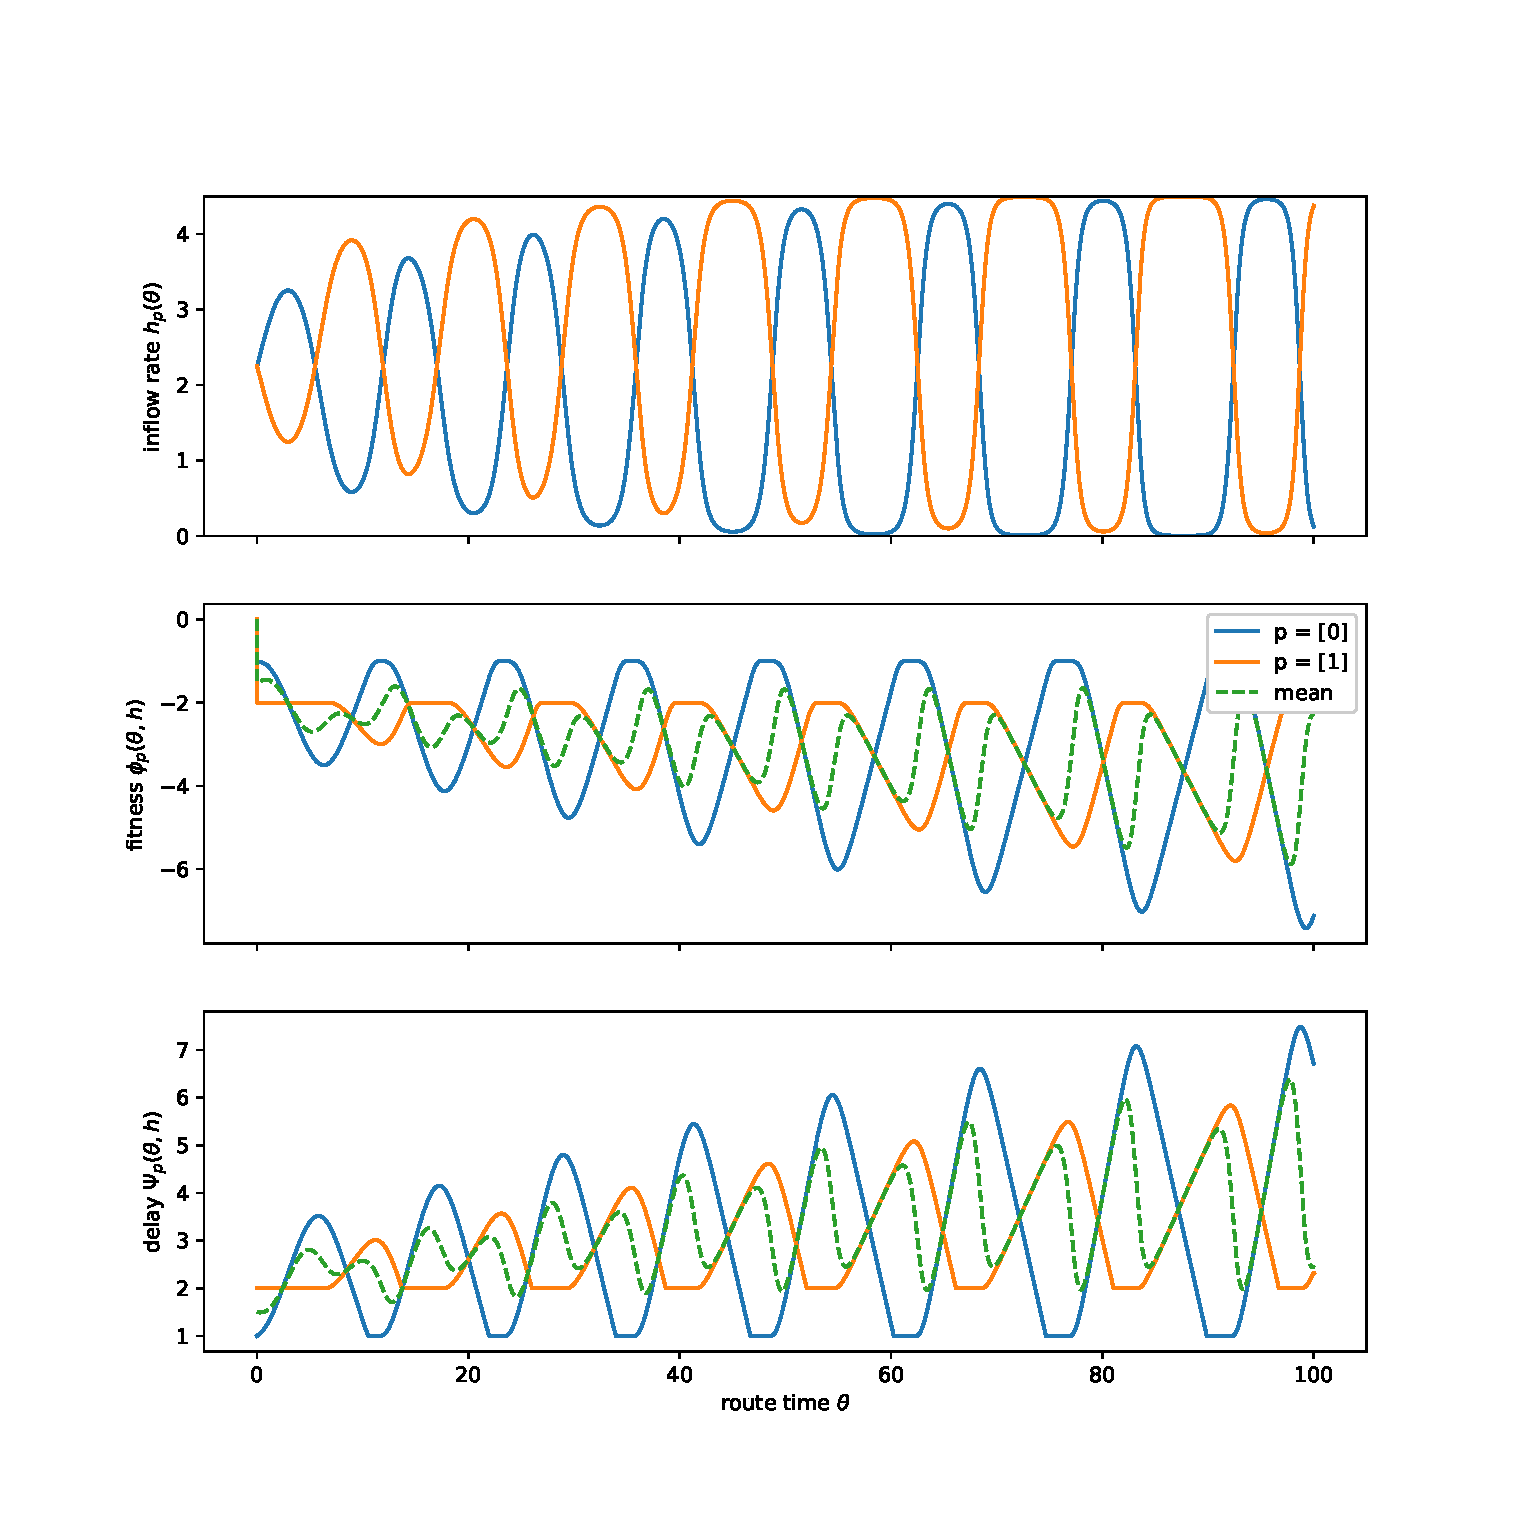
\includegraphics[scale=0.3]{img/pres-replicator_avg_tt.eps}
			\caption{Average delays}	
		\end{figure}	  
	\end{center}  
  
\end{frame}

\begin{frame}
  

	\begin{center}
		\begin{figure}
			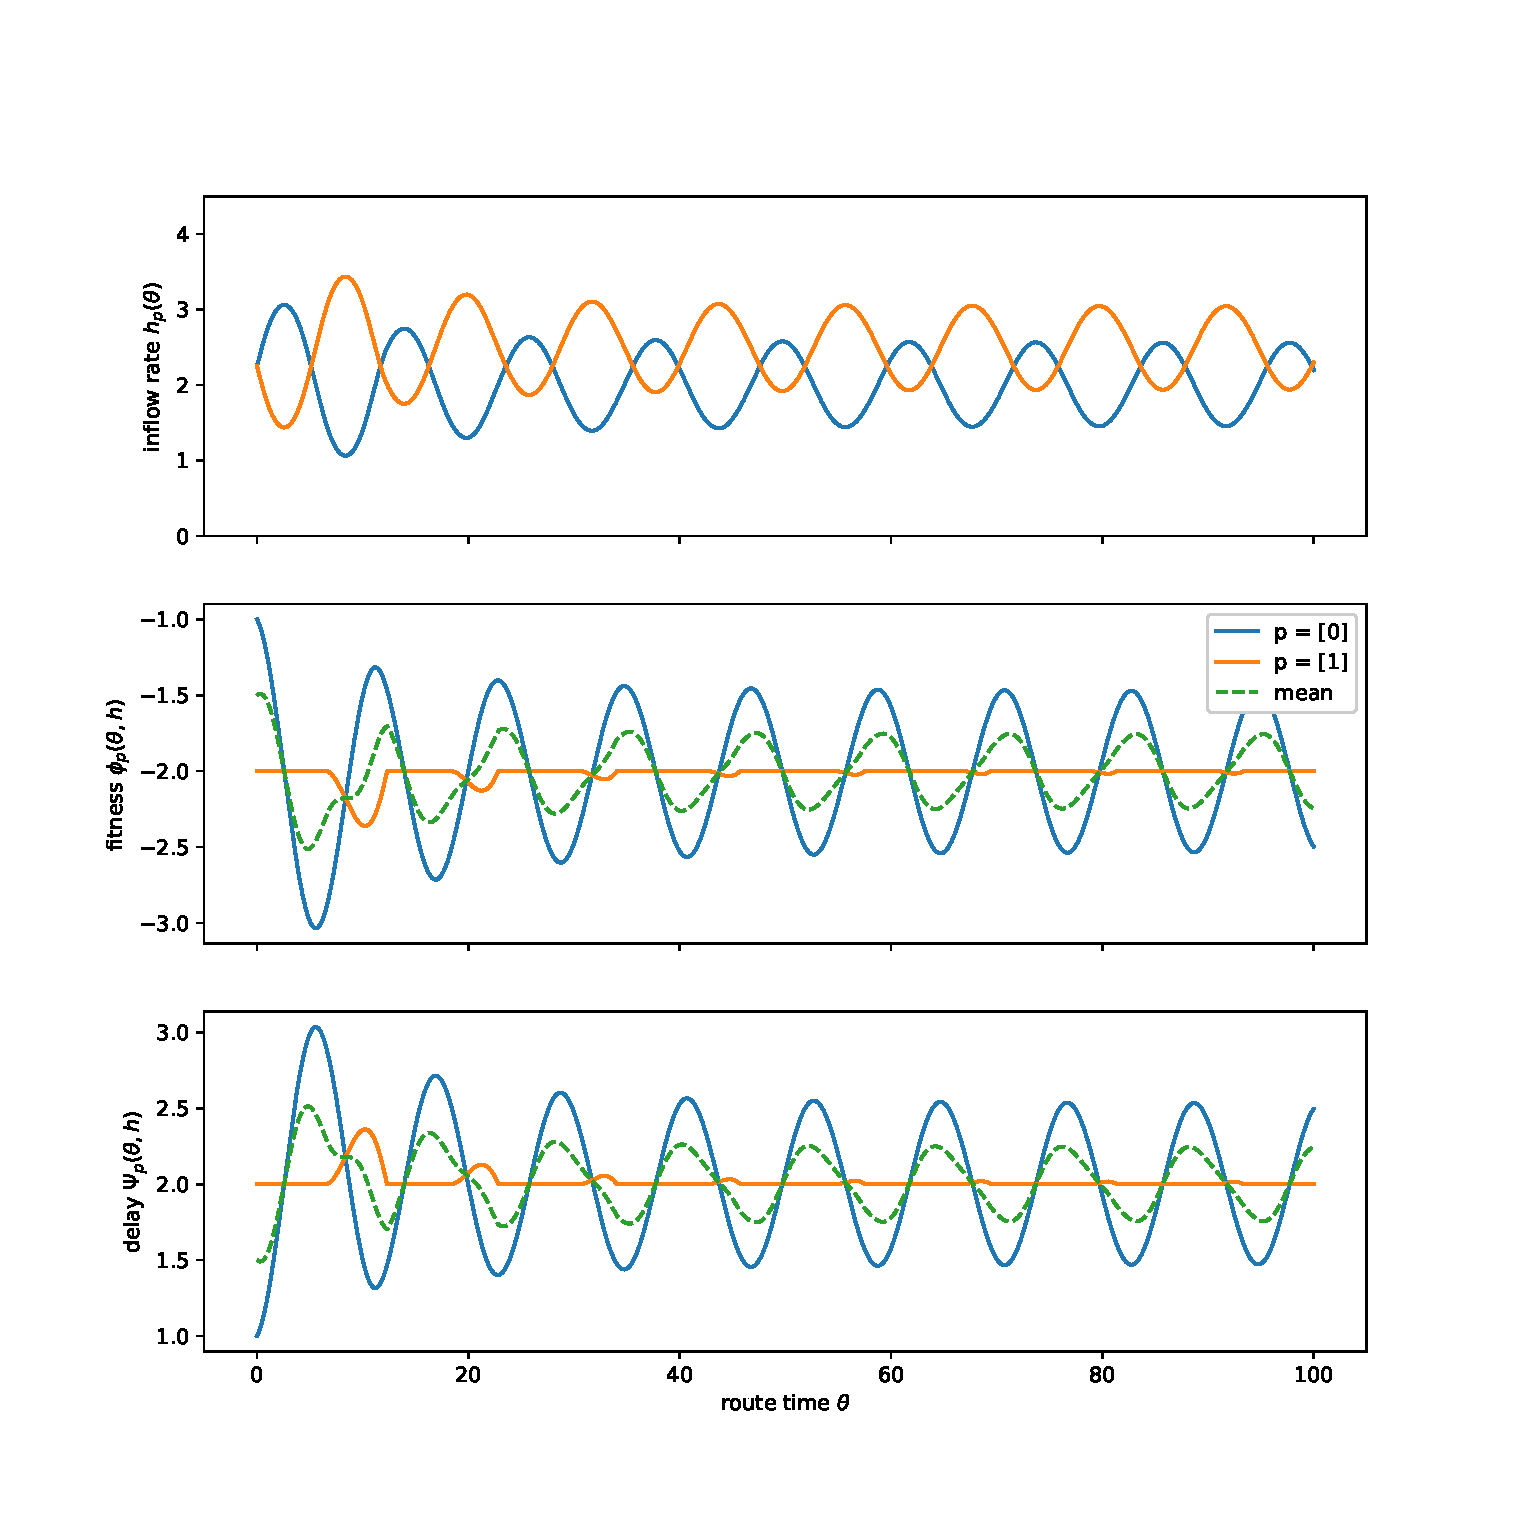
\includegraphics[scale=0.3]{img/pres-replicator_true_tt.eps}
			\caption{True delays}	
		\end{figure}	  
	\end{center}  

\end{frame}

\begin{frame}
  

	\begin{center}
		\begin{figure}
			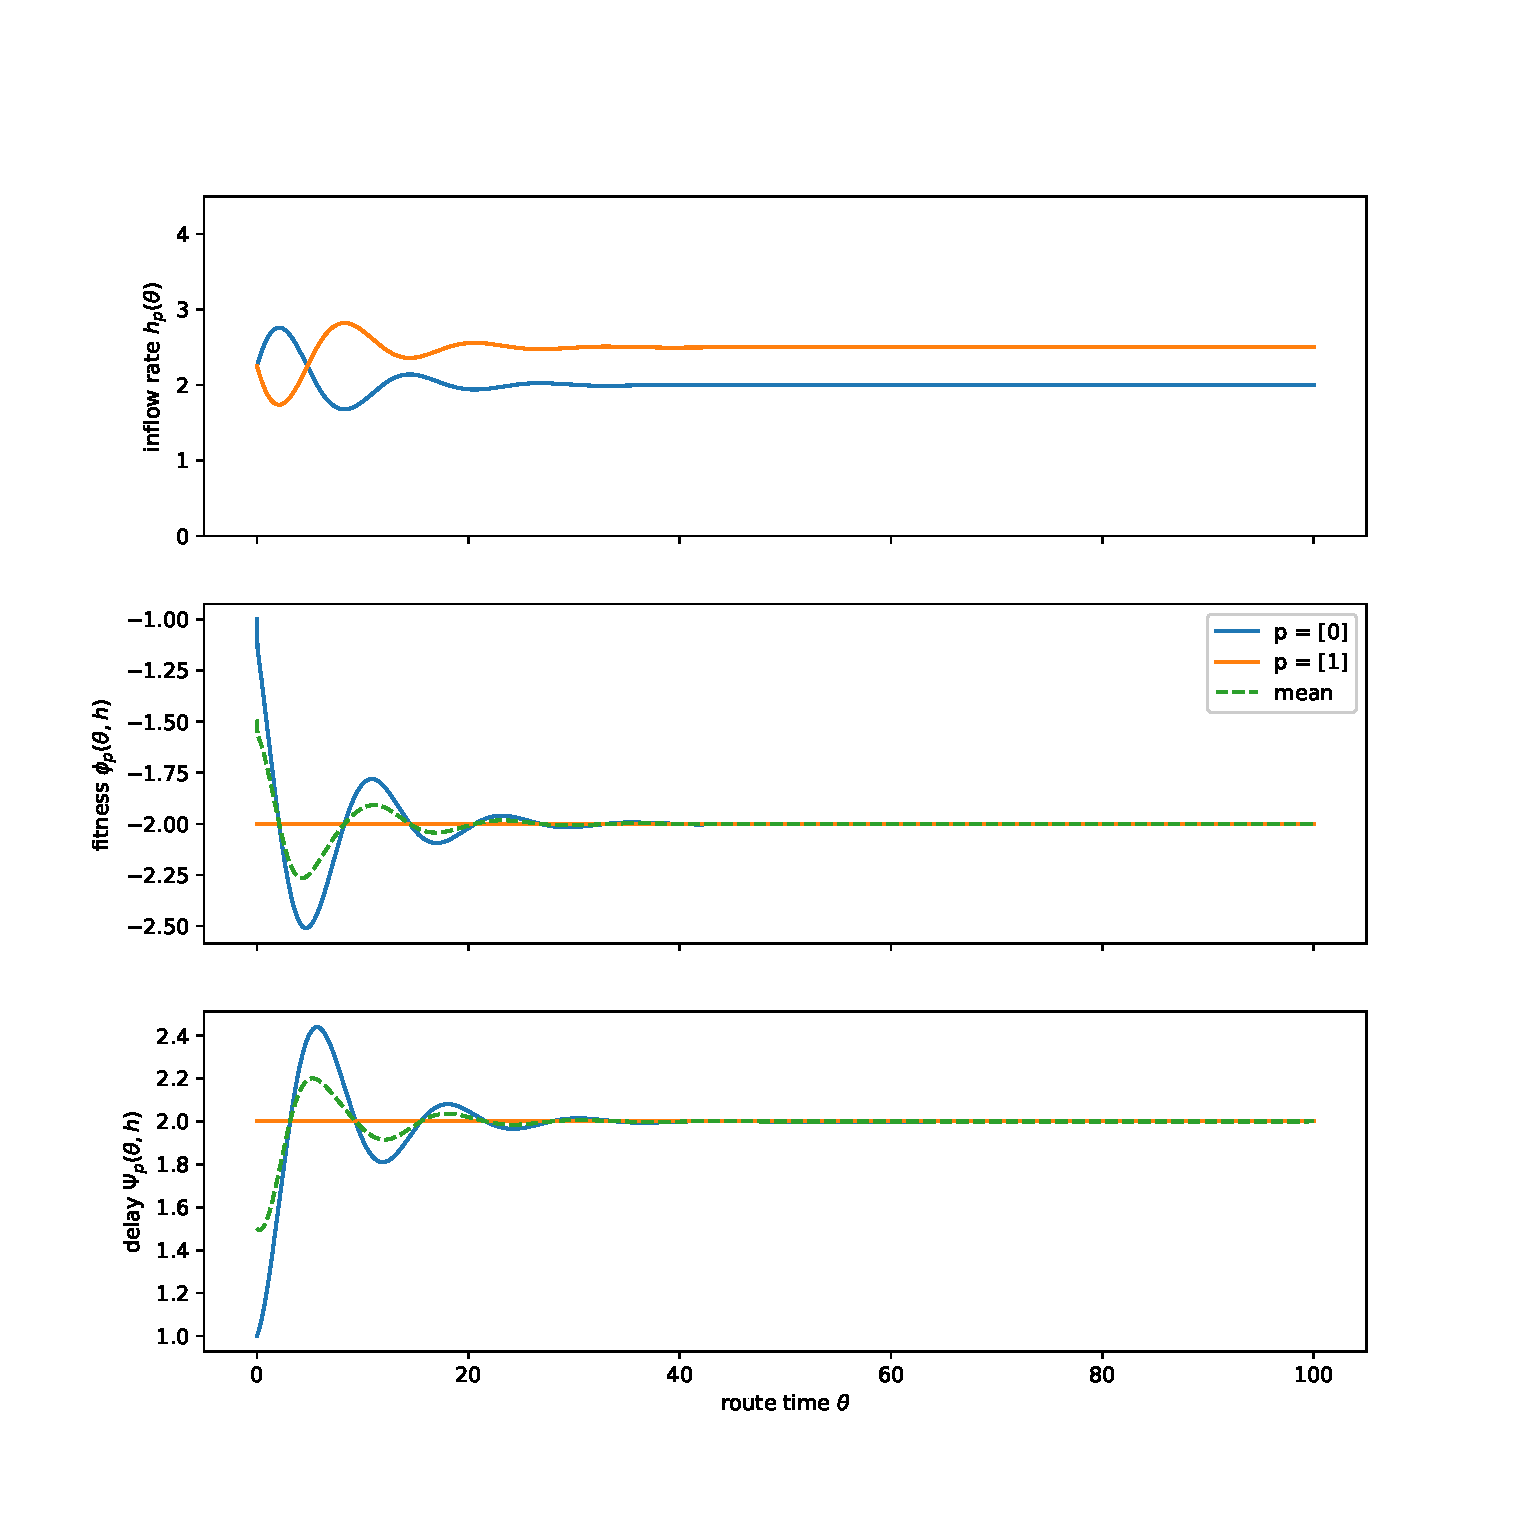
\includegraphics[scale=0.3]{img/pres-replicator_proj_tt.eps}
			\caption{Projected delays}	
		\end{figure}	  
	\end{center}  
  
\end{frame}

\begin{frame}
  

	\begin{center}
		\begin{figure}
			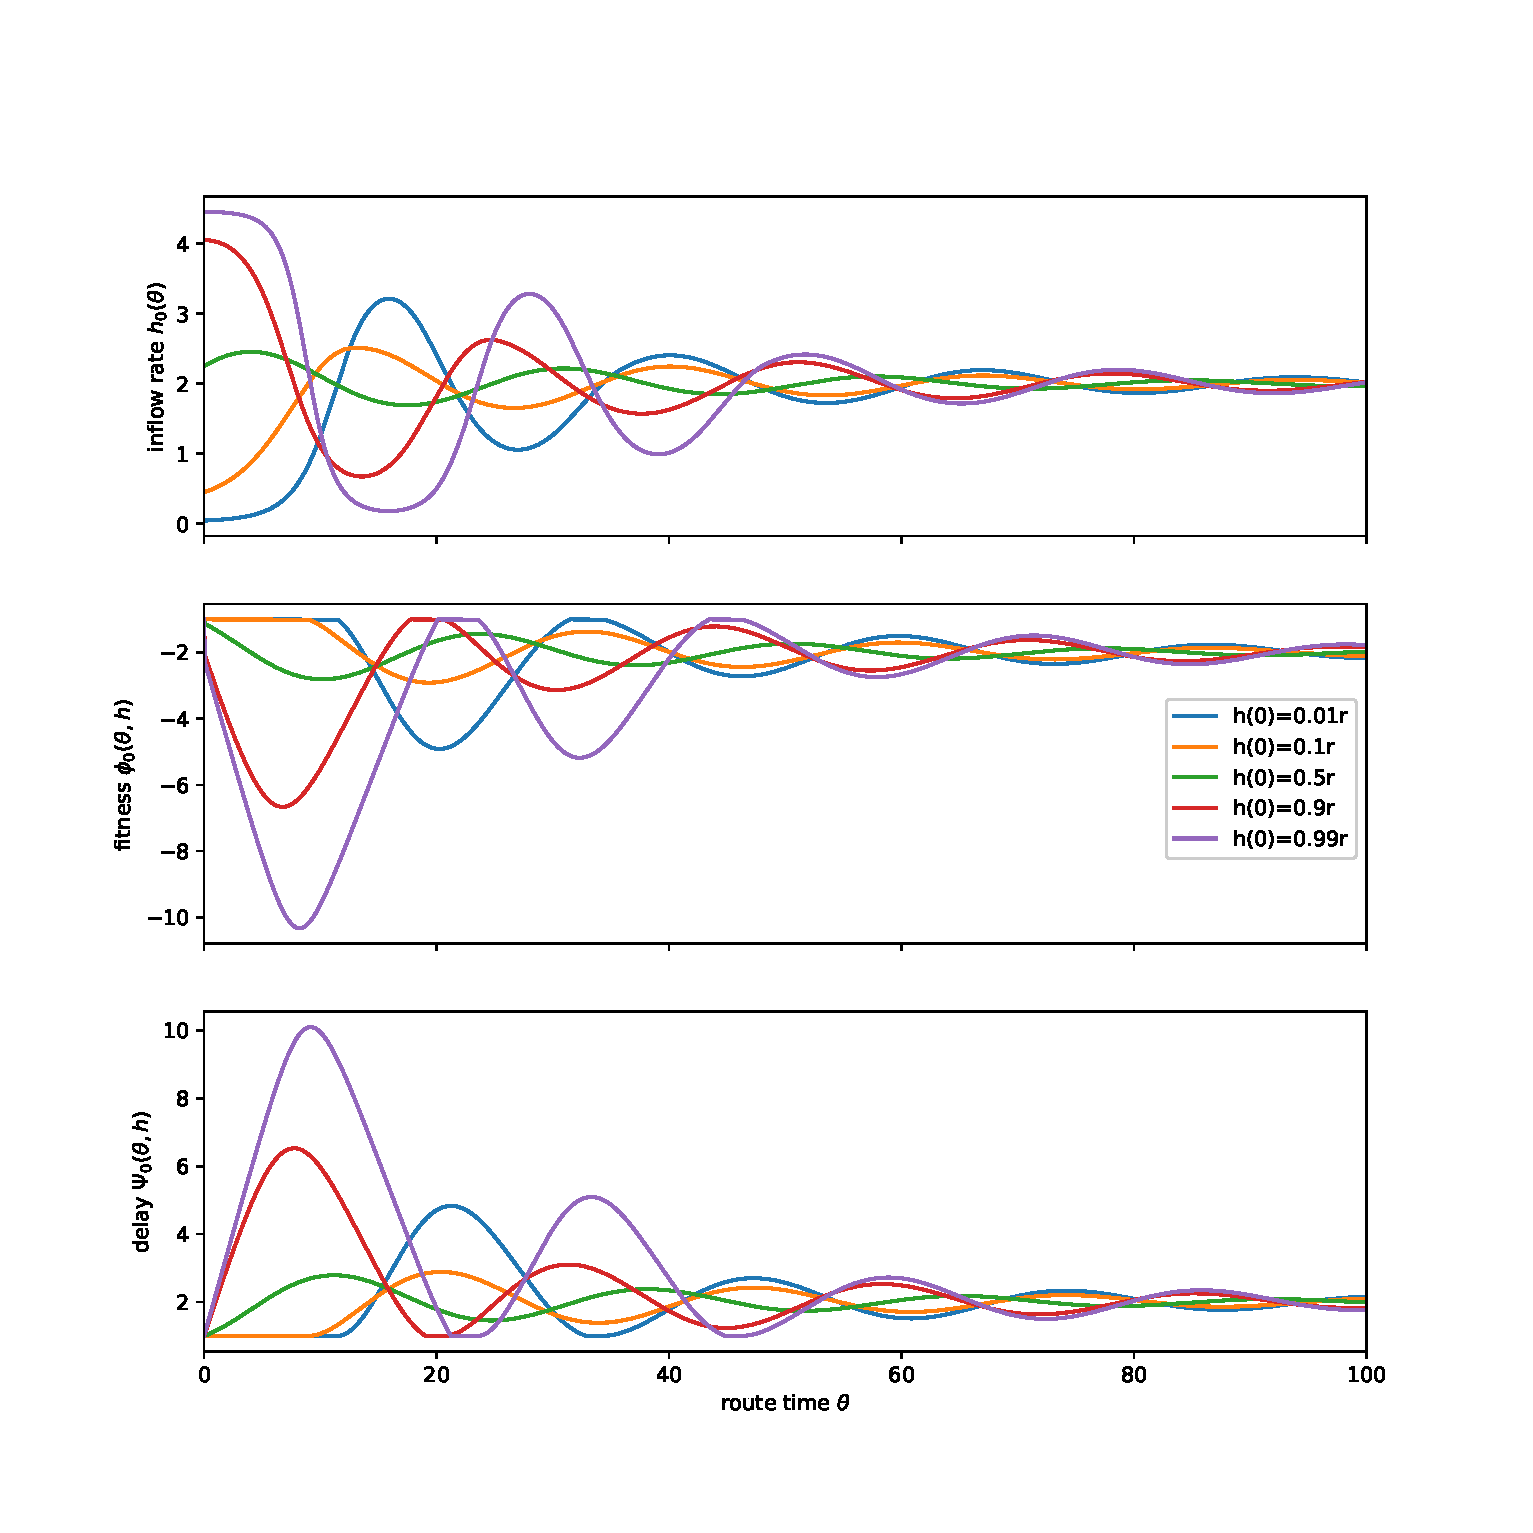
\includegraphics[scale=0.3]{img/pres-replicator_global_stability.eps}
			\caption{Global stability in experiments}	
		\end{figure}	  
	\end{center}  
  
\end{frame}

\section{Analysis}

\subsection{Lyapunov Theory}

\begin{frame}

\subsection*{Lyapunov Theory}

We have an autonomous system $ \dot{x} = f(x), \quad f(0) = 0$ with Lipshitz RHS


\begin{theorem}[Global asymptotic stability]
Let $V: \mathbb{R}^n \to \mathbb{R}$ be a continuously differentiable function, s.t. :
$$V(0) = 0 \text{ and } \forall x \neq 0: ~V(x) > 0  , $$
$$ \lVert x \rVert_2 \to \infty \quad \Rightarrow \quad V(x) \to \infty, $$
$$ \forall x \neq 0 :  ~\dot{V} =  \nabla V(x) \cdot f(x) < 0 $$
Then $x = 0$ is globally asymptotically stable.
\end{theorem}

\begin{theorem}[Local asymptotic stability]
Let $A = \frac{\partial f}{\partial x}(0)$ be Jacobian matrix at $x=0$. If we have $\mathrm{Re} (\lambda_i(A)) < 0$ for all eigenvalues, then $x = 0$ is locally asymptotically stable.

\end{theorem}

\end{frame}

\subsection{Multiple links}

\begin{frame}

\begin{itemize}

\item Consider a network with $n$ parallel links $\{(\tau_i, \nu_i)\}_{i=1}^n$


\item Introduce queue activity indicator $ \mathbb{I}_{q_i} := \begin{cases} 1, & q_i > 0 \text{ or }  h_i \geq \nu_i \\ 0, & \text{otherwise} \end{cases} $ 

\item Fitnesses based on projected delays:

$$ \phi^{proj}_i = - ( \Psi_i + w \dot{\Psi_i} ) = -\left( \tau_i + \frac{q_i}{\nu_i} + w \frac{h_i - \nu_i}{\nu_i} \mathbb{I}_{q_i} \right) $$

\end{itemize}

\end{frame}

\begin{frame}

\begin{itemize}

\item Assumptions:
\begin{enumerate}
	\item strict order $ \tau_1 < \dots < \tau_n$
	\item $ \exists k^* \leq n: ~ \sum_{i=1}^{k^*-1} \nu_i < r < \sum_{i=1}^{k^*} \nu_i $
\end{enumerate}

 
\item There is a unique equilibrium configuration:
$$ \mathbb{I}_{q_i} = \begin{cases} 1 , &i < k^* \\ 0, &i \geq k^*  \end{cases}  \quad \Psi^*_i = \begin{cases} \tau_{k^*}, &i \leq k^* \\ \tau_i, &i > k^*  \end{cases} \quad h^*_i = \begin{cases} \nu_i, &i < k^* \\ r - \sum_{i < k^*} h^*_{i}, &i = k^*\\  0, &i > k^*  \end{cases} $$

\item Any other "instantenious" equillibrium is unstable, i.e. some queues  vanish

\end{itemize}


\end{frame}

\begin{frame}

\begin{itemize}

\item Denote 
\begin{align*}
\Delta q_i &:= \nu_i(\Psi_i - \Psi_i^*) , & 1 \leq i < k^* \\
\Delta h_i &:= h_i - h^*_i, & 1 \leq i \leq n
\end{align*}

\item Assuming same active queues and utilizing $ \sum_{i} \Delta h_i = 0 $  , we linearize the system near the equilibrium :


$$ \frac{d}{d \theta} \begin{bmatrix} \Delta q \\ \Delta h_{< k^*} \\ \Delta h_{k*} \\ \Delta h_{> k^*} \\ \end{bmatrix} \approx \bm{A}
 \begin{bmatrix} \Delta q \\ \Delta h_{< k^*}  \\ \Delta h_{k*} \\ \Delta h_{> k^*} \\ \end{bmatrix} ,$$
 
 $$ \bm{A}  =  -\frac{K}{r} \begin{bmatrix}
 		 0 & -\frac{r}{K} \mathbf{I} & 0 & 0 \\
 		 r \bm{I} - h_{< k^*} \cdot \bm{1}^T  & w ( r\bm{I} - h_{<k^*} \cdot \bm{1}^T ) & 0 & - h_{< k^*} \cdot \tau_{>k^*}^T  \\
 		- h_{k^*} \cdot \bm{1}^T & 0 &  w h_{k^*} & - h_{k^*} (\tau_{>k^*} - w \bm{1})^T \\
 		 0 & 0 & 0 & r (\mathrm{diag}(\tau_{>k^*}) - \tau_{k^*} \bm{I}) )  \\
 		 
  \end{bmatrix} $$


\end{itemize}

\end{frame}



\begin{frame}

\begin{itemize}

\item Finding eigenvalues by $ \bm{A} v = \lambda v$ with $v =  \begin{bmatrix} a & b & c & d \end{bmatrix}^T $

\begin{enumerate}

\item $c, d = 0$:

$  -\frac{K}{r} (r \bm{I} - h_{< k^*} \cdot \bm{1}^T) a = \mu a$  $ \Rightarrow$ $ \quad \mu = -K$ or $\mu = -K  (1 - \frac{1}{r}\bm{1}^T h_{< k^*}) < 0 $
\\
$\lambda^2 = \mu (1 + w \lambda)$ $\Rightarrow$ $Re(\lambda) < 0$

\item $c \neq 0$: $h_{k^*} > 0 $ $\Rightarrow $ $\lambda < 0$

\item $d \neq 0$: $\tau_j > \tau_{k^*}$ for $j > k^*$ $\Rightarrow $ $\lambda < 0$


\end{enumerate}



\item We have $\mathrm{Re}( \lambda(\bm{A}) ) < 0$, which guarantees local asymptotic stability


\end{itemize}

\end{frame}

\begin{frame}

	\begin{center}
		\begin{figure}
			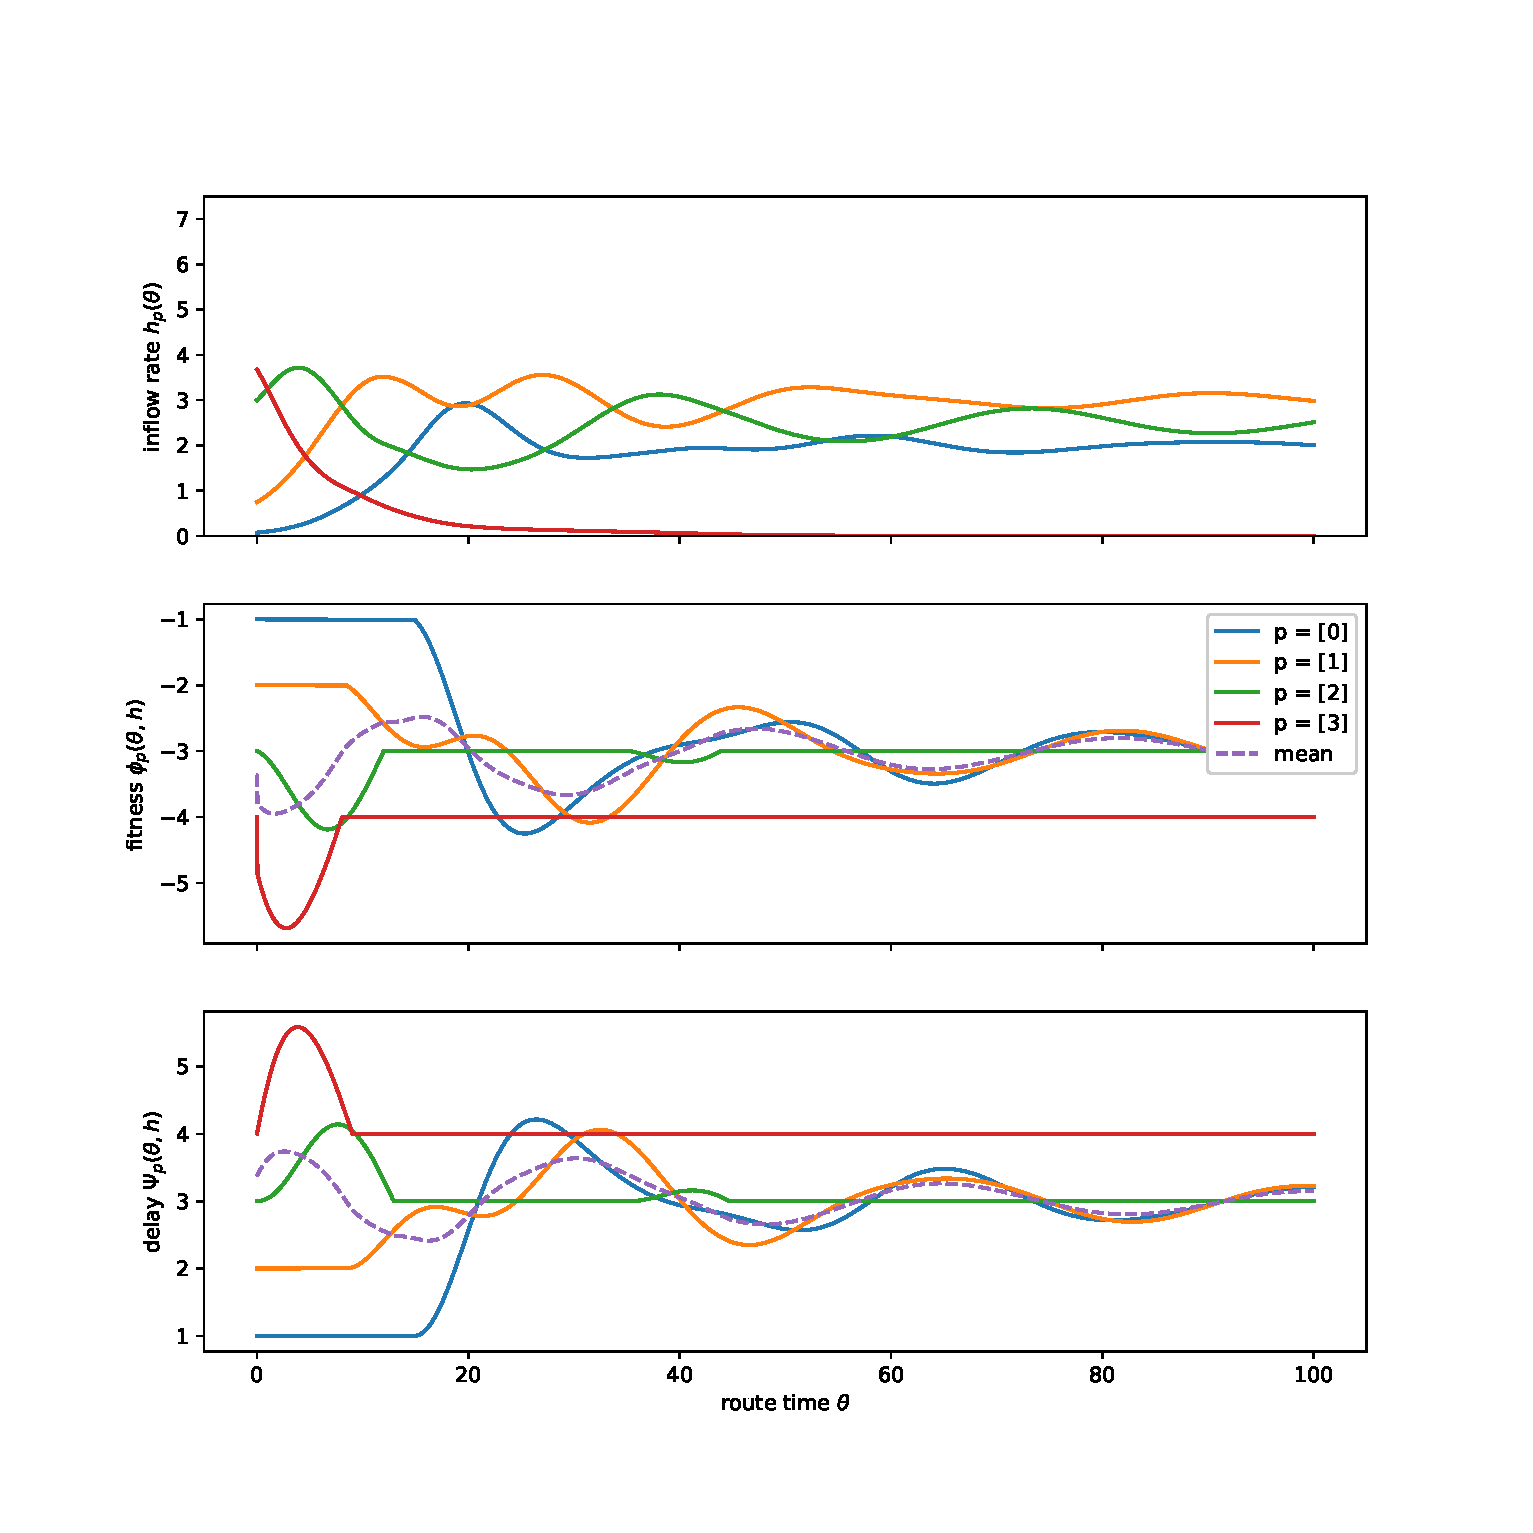
\includegraphics[scale=0.3]{img/pres-replicator_more_links.eps}
			\caption{Multiple links}	
		\end{figure}	  
	\end{center}  
  

\end{frame}



\subsection{Two links}

\begin{frame}

\begin{itemize}

\item Suppose we only have two links 0 and 1 with $\tau_0 < \tau_1$. 

\item Denoting $ \psi(\theta, h) := \Psi_0(\theta, h) - \Psi_1(\theta, h) $ allows to simplify the equations:

\begin{align*}
	\dot{h_0} &= - \frac{K}{r} h_0 (r - h_0) ( \psi + w \dot{\psi} ) \\
	\dot{\psi} &= \frac{h_0 - \nu_0}{\nu_0} \mathbb{I}_{q_0} + \frac{ h_0  - (r - \nu_1)}{\nu_1} \mathbb{I}_{q_1}
\end{align*}


\item Equillibrium  $\Leftrightarrow$  $ \psi, \dot{\psi} = 0$


\end{itemize}


\end{frame}

\begin{frame}

\begin{itemize}

 

\item Introduce inflow potentials

$$ \Pi_0(h_0) := \int_{\nu_0}^{h_0} \frac{ r \frac{h - \nu_0}{\nu_0} }{h(r-h)} dh, \quad \Pi_1(h_0) := \int_{ r-\nu_1}^{h_0}  \frac{ r \frac{h - (r - \nu_1)}{\nu_1} }{h(r-h)} dh $$

\item Candidate for Lyapunov function 
$$ V(\psi, h_0) = \frac{1}{2}\psi^2 + \frac{1}{K} \left( \Pi_0 \mathbb{I}_{q_0} + \Pi_1 \mathbb{I}_{q_1} \right) $$

\begin{enumerate}

\item $V = 0$ only at the equilibrium, else $V > 0$;

\item $V \to \infty$ if $|\psi| \to \infty$ or $h_0 \to 0,1$;

\item For each queue configuration we have
$$ \dot{V} = \frac{\partial V}{\partial \psi} \dot{\psi} + \frac{\partial V}{\partial h_0} \dot{h_0}  = -w \dot{\psi}^2 \leq 0$$

\end{enumerate}


\item Problem: switching between cases

\end{itemize}

\end{frame}

\begin{frame}


	
	\begin{center}
		\begin{figure}
			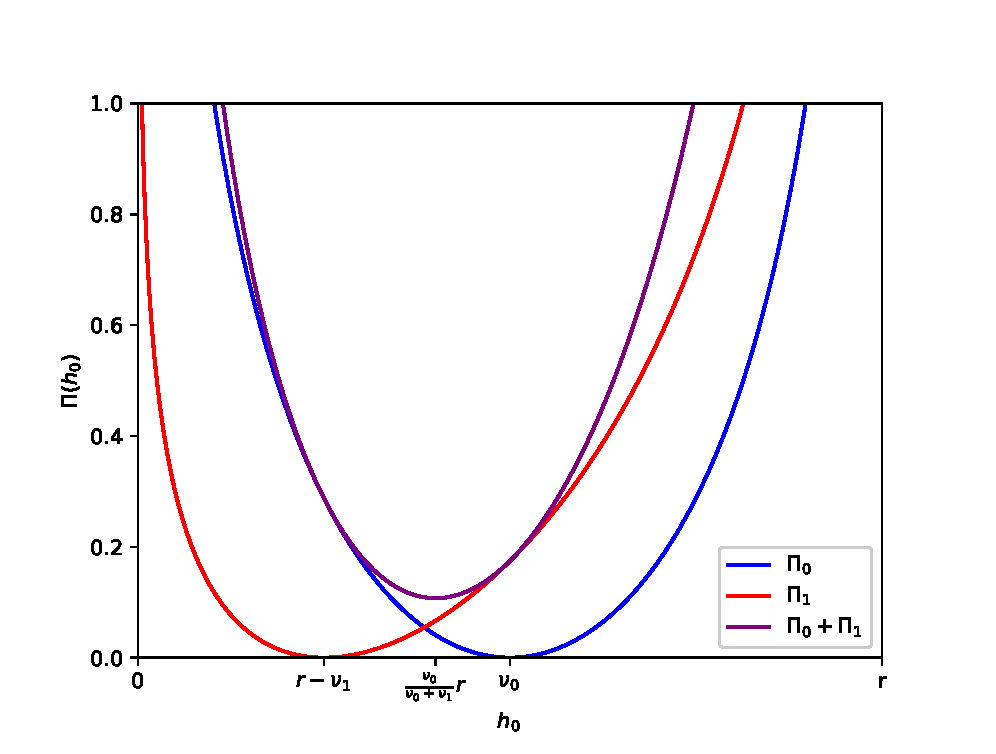
\includegraphics[scale=0.6]{img/potentials.eps}
			\caption{Inflow potentials}	
		\end{figure}	  
	\end{center}  

 
\end{frame}

\begin{frame}
 
 		\begin{center}
		\begin{figure}
			
		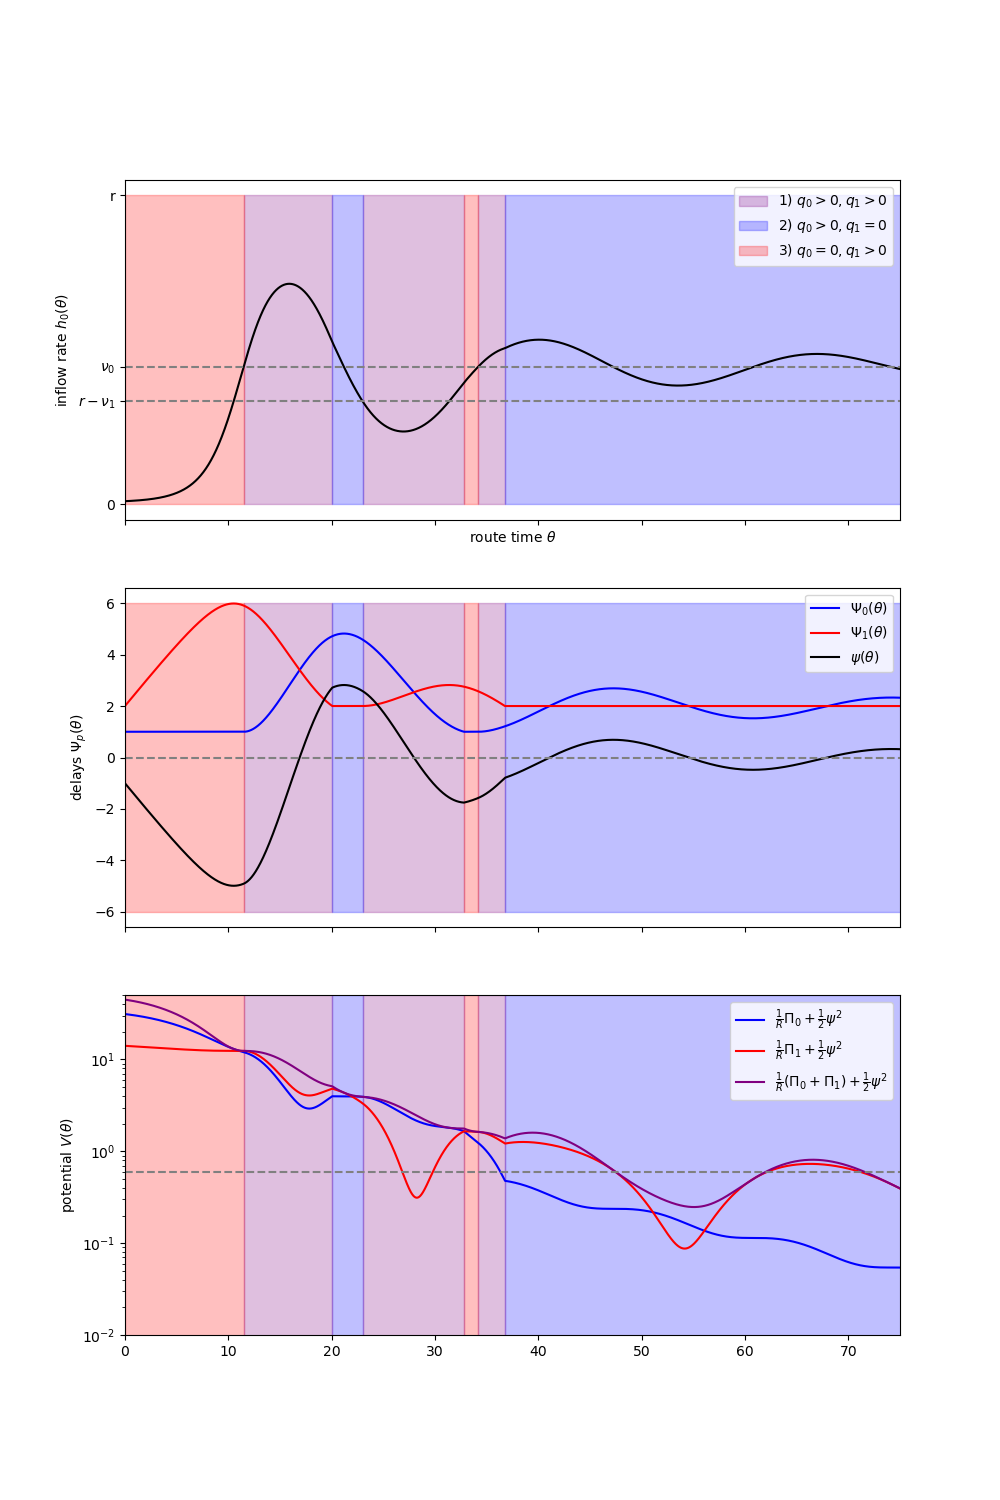
\includegraphics[scale=0.25]{img/phases.png}
		\caption{Case switching}	
		\end{figure}	  
	\end{center}  
	
 
\end{frame}


\begin{frame}


\begin{itemize}

\item Max demand: $r = \nu_0 + \nu_1$

\item Three different "attractors" merge into one
$$ r - \nu_1 = r \frac{ \nu_0}{\nu_0 + \nu_1} = \nu_0 $$

\item Denote $ Q := q_0 + q_1 $ and observe that
$$ \dot{Q} = \dot{q_0} + \dot{q_1} = \left( h_0 - \nu_0 \right) \mathbb{I}_{q_0} +  \left( (r - h_0) - \nu_1 \right) \mathbb{I}_{q_1} \geq 0 $$

\item Queues grow and can't vanish 
$$ \Psi_e(\theta, h) - \Psi_e(\theta, h^*) \stackrel{\theta \to \infty}{\to} c > 0$$

\end{itemize}

\end{frame}

\begin{frame}


	\begin{center}
		\begin{figure}
			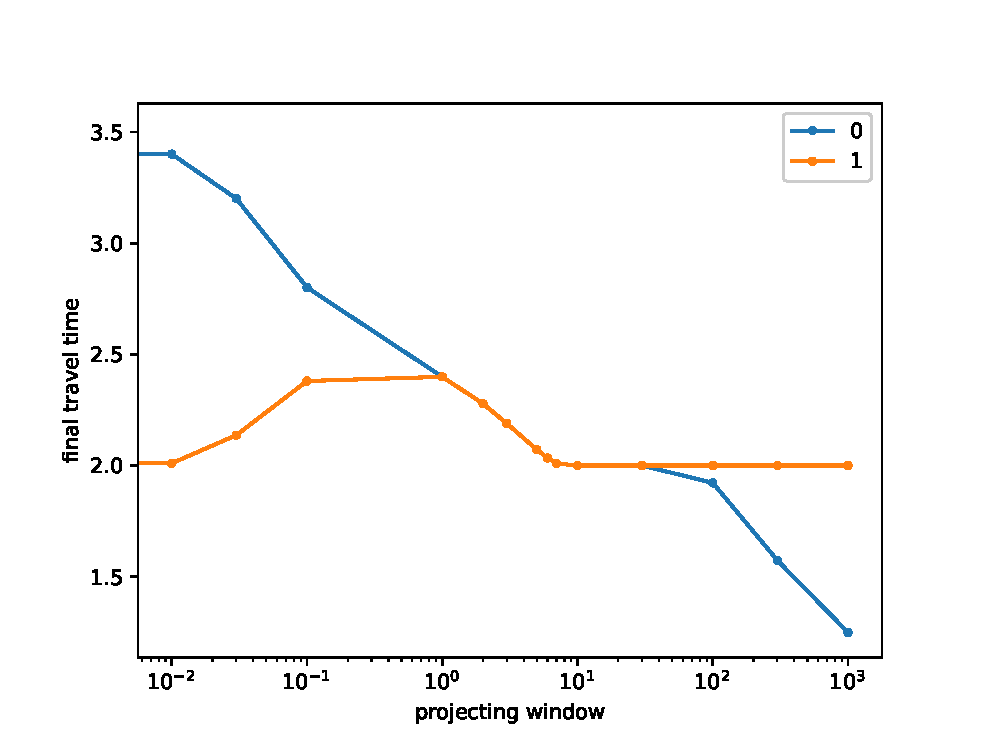
\includegraphics[scale=0.5]{img/final_tt_proj.eps}
		\caption{Max demand convergence}	
		\end{figure}	  
	\end{center}  

 

\end{frame}


\section{Further directions}

\begin{frame}

\begin{itemize}
\item Showing global stability
	\begin{enumerate}
	
	\item Patterns in case switching	
	
	\item Max demand 	
	
	\end{enumerate}
	
\item Considering more complex networks

\item Other options for fitnesses

\end{itemize}

\end{frame}

\end{document}